\documentclass[11pt]{article}
\usepackage[sc]{mathpazo} %Like Palatino with extensive math support
\usepackage{fullpage}
\usepackage[authoryear,sectionbib,sort]{natbib}
\linespread{1.7}
\usepackage[utf8]{inputenc}
\usepackage{lineno}
\usepackage{titlesec}
\titleformat{\section}[block]{\Large\bfseries\filcenter}{\thesection}{1em}{}
\titleformat{\subsection}[block]{\Large\itshape\filcenter}{\thesubsection}{1em}{}
\titleformat{\subsubsection}[block]{\large\itshape}{\thesubsubsection}{1em}{}
\titleformat{\paragraph}[runin]{\itshape}{\theparagraph}{1em}{}[. ]\renewcommand{\refname}{Literature Cited}

% Added packages
\usepackage{amsmath} % for matrices
\usepackage{graphicx} % for organizing figures
\usepackage{lmodern} % for tilde
\usepackage[T1]{fontenc} % for tilde

%%%%%%%%%%%%%%%%%%%%%
% Line numbering
%%%%%%%%%%%%%%%%%%%%%
%\usepackage{lineno}
% Please use line numbering with your initial submission and
% subsequent revisions. After acceptance, please turn line numbering
% off by adding percent signs to the lines %\usepackage{lineno} and
% to %\linenumbers{} and %\modulolinenumbers[3] below.

\title{TBD}
% 1. Populations experience fewer selective constraints in complex food webs
% 2. Complex food webs impose fewer selective constraints on linked populations
% 3. Food-web complexity reduces selective constraints on an insect herbivore
% 4. Phenotypic evolution is less constrained in complex food webs

% This version of the LaTeX template was last updated on
% January 11, 2018.

%%%%%%%%%%%%%%%%%%%%%
% Authorship
%%%%%%%%%%%%%%%%%%%%%
% Please remove authorship information while your paper is under review,
% unless you wish to waive your anonymity under double-blind review. You
% will need to add this information back in to your final files after
% acceptance.

\author{Matthew A. Barbour$^{1,2,\ast}$ \\ 
Christopher J. Greyson-Gaito$^{1,3}$ \\ 
Arezoo Sootodeh$^{3}$ \\
Brendan Locke$^{4} \\
Jordi Bascompte$^{2}}

\date{}

\begin{document}

\maketitle

\noindent{} 1. University of British Columbia, Department of Zoology, Vancouver, British Columbia V6T 1Z4, Canada;

\noindent{} 2. University of Zurich, Department of Evolutionary Biology and Environmental Studies, Winterthurerstrasse 190, 8057 Zurich, Switzerland;

\noindent{} 3. University of Guelph, Department of Integrative Biology, Guelph, Ontario N1G 2W1, Canada;

\noindent{} 3. Humboldt State University, Department of Biological Sciences, Arcata, California 95521, USA.

\noindent{} $\ast$ Corresponding author; e-mail: matthew.barbour@ieu.uzh.ch.

\bigskip

\textit{Manuscript elements}: Figure~1, figure~2, figure~3. All figures should be printed in color.

\bigskip

\textit{Keywords}: Adaptive landscape, host-parasitoid, natural selection, G-matrix.

\bigskip

\textit{Manuscript type}: Article. %Or e-article, note, e-note, natural history miscellany, e-natural history miscellany, comment, reply, invited symposium, or countdown to 150.

\bigskip

\noindent{\footnotesize Prepared using the suggested \LaTeX{} template for \textit{Am.\ Nat.}}

\linenumbers{}
\modulolinenumbers[3]

\newpage{}

\section*{Abstract}



\newpage{}

\section*{Introduction}

% The journal does not have numbered sections in the main portion of
% articles. Please refrain from using section references (à la
% section~\ref{section:CountingOwlEggs}), and refer to sections by name
% (e.g. section ``Counting Owl Eggs'').


% I. Adaptive landscape is a powerful framework for understanding the evolution of biological diversity (or phenotypic evolution).

The adaptive landscape provides a powerful framework for understanding and predicting the evolution of biological diversity \textemdash from genes, to phenotypes, to species (Wright and Simpson). More than a metaphor, the adaptive landscape links quantitative genetic and phenotypic variation to evolution by natural selection (Lande 1979, Arnold papers). In particular, the shape of the adaptive landscape represents the presence and strength of different selection pressures imposed by the environment (Arnold's work). Species interactions often play a key role in defining the selective environment, as evidenced by the influence of resource competition (Schluter 2000), mutualisms (Jordano 1987), and predation (Abrams 2000) on the evolution of biological diversity. Although there is clear evidence that pairwise interactions shape the adaptive landscape, we also know that most species interact with multiple species in an ecological community. Understanding how the adaptive landscape is shaped by community context represents a major challenge for both empiricists and theoreticians given the diversity of selection pressures that a population is likely to experience in a natural ecological community. 

% II. Species-interaction networks provide an explicit representation of the community context that populations are embedded within.

Species-interaction networks, such as a food web describing who eats whom, provide an explicit representation of the community context. These networks describe the interdependency of species within an ecological community, providing an effective framework for predicting how changes in the density of directly and indirectly connected species will impact other species, and in turn, community dynamics. Despite the importance of species-interaction networks for predicting ecological dynamics, these networks often lack quantitative information on how species interactions influence natural selection. Consequently, it is unclear how species-interaction networks shape the adaptive landscape, creating a major hurdle in our current ability to predict how changes in community context will affect phenotypic evolution. 

% III. Here we combine these frameworks to predict how changes in community context will affect phenotypic evolution. (empirically?)

Here, we integrate species-interaction networks and the adaptive landscape to predict how changes in network structure will affect phenotypic evolution. We did this by conducting a field experiment to characterize the effect of network structure on the adaptive landscape of a constituent species. Specifically, we conducted a field experiment that manipulated the diversity of insect parasitoids that were able to impose selection on an abundant insect herbivore (\textit{Iteomyia salicisverruca})(Fig. 1). The larva of this herbivore species induce tooth-shaped galls when they feed on the developing leaves of willow trees (\textit{Salix} sp., @Russo2006). These galls provide protection from generalist predators (e.g. ants, spiders), thus the network of interacting parasitoids provides a realistic representation of the biotic environment this insect herbivore is experiencing. Therefore, our manipulation of parasitoid diversity alters the diversity of interactions, or food-web complexity, that this insect herbivore experiences.

% IV. Lay out predictions for how changes in network structure influence the adaptive landscape.

Changes in food-web complexity could influence a resource population's adaptive landscape in at least two ways. First, if a more diverse community of consumers is more effective at suppressing resource densities (@Ives2005), then this will result in lower mean fitness of the resource population. A reduction in mean fitness, all else equal, will intensify natural selection (@Hunter2018). On the other hand, if consumers impose different selection pressures on resource traits, then more diverse communities could dampen the strength of selection acting on a given trait. This is because a greater diversity in selection pressures is equivalent to greater uncertainty in the selective environment. Thus, a more diverse consumer community may relax the net selection pressures acting on resource traits. Here, we evaluate these hypothesized relationships through an experimental test of how changes in food-web complexity alters the adaptive landscape of a resource population.

% Confronting this challenge is important now more than ever before, given the rapid changes we are witnessing in the diversity and composition of local communities (cite global change papers).

% Natural selection is inherently an ecological process, describing how the environment changes phenotypic distributions of a population due to differences in fitness. %within a generation
 
%At the same time, evolutionary biologists have long recognized that changes in the biotic environment can alter the dynamics of natural selection. However, the biotic environment in which populations are evolving often remains a bit of a "black box" that's labelled by a general ecological process such as competition, predation, or mutualism. Because of this, it remains difficult to predict how changes in the biotic environment will affect the direction and magnitude of natural selection. Such predictions are urgently needed given the rapid changes in the biotic environment that most populations are currently experiencing throughout the world. 

% For example, the Lande equation ($\delta z=G\beta$) predicts the evolutionary trajectory of phenotypes ($\delta z$) as a function of directional selection gradients ($\beta$) and the additive genetic variance and covariance between these phenotypes (G-matrix, $G$). Similarly, the curvature of the adaptive landscape ($\gamma - \beta \beta^\text{T}$). also shapes the G-matrix, which ultimately determines the ... . Importantly, the components of this theoretical framework can be est quantities that predict evolutionary change can all be estimated empirically

% People have often studied pairwise species interactions. There is also tantalizing evidence that community context can alter natural selection on phenotypic distributions, but predicting these changes remains difficult. This is because work hasn't explicitly embodied the environment (which a network can).

% Key part here is environment, which a food web or species-interaction network can provide an explicit representation of (i.e. community context).

% Biological diversity \textemdash from genes, to phenotypes, to species \textemdash has and continues to be shaped by the interplay between ecological and evolutionary processes. Much of this biological diversity has been molded by natural selection arising from species interactions, such as resource competition (Schluter 2000), mutualisms (Jordano 1987), and predation (Abrams 2000). While there is clear evidence that pairwise interactions can drive evolution, we also know that most species interact with multiple species in an ecological community. Understanding and predicting how evolutionary dynamics unfold in a community context represents a major challenge both empirically and theoretically, given the diversity of selection pressures that a population is likely to experience in an ecological community. Answering this question also has important applications, especially given the rapid changes we are witnessing in the diversity and composition of local communities (cite global change papers). 

% is a key challenge and predicting how changes in ecological communities is challenging and eminently theoretical (@McPeek2017, @De_Mazancourt2008, @Guimaraes2017, @Nuismer2013). 


%<!-- Do I need to give more credit here to work by @TerHorst2018 and others?). I think it would be useful to show that there is some field and lab experiments demonstrating that community context can alter evolutionary trajectories -->
%<!-- Given the rapid loss of species diversity we are experiencing throughout the world (cite), we are in urgent need of work that makes and tests predictions for how the loss of species will affect the evolutionary process in natural communities.

%<!-- Theoretical models have begun to examine how the network structure of species interactions drives evolutionary change (Nuismer paper; Guimeras paper; Ecology Letters paper from a spanish guy...; @McPeek2017); however, we are currently lacking experimental tests of how changes in network structure will alter the dynamics of natural selection in the field. -->

% The fitness landscape provides a unifying framework for linking the ecology and evolution of populations (Lande 2007; McPeek 2017). The average fitness of a population is a common currency in ecology and evolution, but usually goes by different names in each field. Ecologists refer to it as per-capita population growth rate ($dN/Ndt$), whereas evolutionary biologists call it the natural log of population mean fitness ($ln(\bar W_N)$). In addition to having different names, ecologists and evolutionary biologists have typically focused on different processes that shape the fitness landscape. For example, population ecologists have long studied the effect of a population's density on its per-capita growth rate (i.e. density-dependence, CITE Foundational and current work). In contrast, evolutionary biologists have focused on how the mean trait value of a population influences its average fitness, as this describes the direction and magnitude of natural selection (CITE foundational and current work). Therefore, the fitness landscape describes the joint ecological and evolutionary dynamics of a population in a given environment.

% Community ecologists have extended the ecological side of the fitness landscape by incorporating network theory. Species-interaction networks, such as a food web describing who eats whom, provide an explicit representation of the biotic environment as they describe the interdependency of populations within an ecological community. This has provided an effective framework for predicting how changes in the biotic environment (e.g. density of directly and indirectly connected species) will impact population dynamics within species-rich communities. At the same time, evolutionary biologists have long recognized that changes in the biotic environment can alter the dynamics of natural selection. However, the biotic environment in which populations are evolving often remains a bit of a "black box" that's labelled by a general ecological process such as competition, predation, or mutualism. Because of this, it remains difficult to predict how changes in the biotic environment will affect the direction and magnitude of natural selection. Such predictions are urgently needed given the rapid changes in the biotic environment that most populations are currently experiencing throughout the world. 


\section*{Methods}

\subsection*{Study Site}

We conducted our study within a four-year old common garden of coastal willow (\textit{Salix hookeriana}) located at Humboldt Bay National Wildlife Refuge (HBNWR) (40\textdegree 40'53"N, 124\textdegree 12'4"W) near Loleta, California, USA. This common garden consists of 26 different willow genotypes that were collected from a single population of willows growing around Humboldt Bay. Stem cuttings of each genotype (25 replicates per genotypes) were planted in a completely randomized design in two hectares of a former cattle pasture at HBNWR. Willows in our garden begin flowering in February and reach their peak growth in early August. During this study, willows had reached 5 - 9m in height. Further details on the genotyping and planting of the common garden are available in @Barbour2015.  

\subsection*{Food-web Manipulation}

We setup our food-web manipulation across 128 plants soon after galls began developing on *S. hookeriana* in early June of 2013. 
These 128 plants came from eight different plant genotypes, spanning the range of trait variation observed in this willow population (@Barbour2015). 
On treatment plants (8 replicates per genotype), we enclosed 14 galled leaves with 10x15cm organza bags (ULINE, Pleasant Prairie, WI, USA) to exclude three parasitoid species that attack during larva development (hereafter larval parasitoids). 
This treatment did not exclude the egg parasitoid *Platygaster* sp. which attacks prior to gall initiation (note that in Cecidomyiid midges, larva initiate gall development CITE). 
On control plants (8 replicates per genotype), we used flagging tape to mark 14 galled leaves per plant (~30 larva), allowing the full suite of parasitoids to attack \textit{Iteomyia}. 
Marking galls with flagging tape ensured that we compared control and treatment galls with similar phenology when we collected galls later in the season. 
Our food-web manipulation altered the average number of trophic interactions that \textit{Iteomyia} was exposed to from BLANK on control plants to BLANK on treatment plants. 
Thus, we refer to galls on control plants as being exposed to a 'complex' food web, whereas galls on treatment plants were exposed to a 'simple' food web.
In late August, we collected marked and bagged galls from each plant, placed them into 30 mL vials and kept them in the lab for 4 months at room temperature. 
We then opened galls under a dissecting scope and determined whether larva survived to pupation (our measure of fitness) or were parasitized. Since we were interested in selection imposed by interactions with parasitoids, we restricted our data to larva that either survived to pupation, was parasitized by an egg parasitoid (\textit{Platygaster} sp.), or was parasitized by a larval parasitoid. For the food-web treatment that excluded parasitoids, we further restricted our data by removing any instances of parasitism by a larval parasitoid. This represented less than 3\% of the observations in this food-web treatment and allowed us to focus our inferences of selection on those imposed by the egg parasitoid.  
Together, we had survival estimates for 1,306 larva from 607 galls, 111 plants, and 8 plant genotypes.

\subsection*{Measuring Gall Traits}

We collected data on three different traits that we anticipated would experience selection based on our previous work (@Barbour2016) and others work with Cecidomyiid midges (@Weis1983, @Heath2018) (\citealt{Heath2018}). 
First, we measured gall diameter as the size of each gall chamber to the nearest 0.01 mm at its maximum diameter (perpendicular to the direction of plant tissue growth). 
Our previous work has shown that a larger gall diameter provides a refuge for larva from parasitoid attack (@Barbour2016). <!-- Consider whether it is important to make the distinction that diameter was measured at the multi-chambered gall level in previous work -->
Second, we measured the clutch size of adult female midges by counting the number of chambers in each gall (@Weis1983). 
All larva collected from the same multi-chambered gall were scored with the same clutch size. 
Third, we measured female preference for oviposition (egg-laying) sites as the density of larva observed on a plant in an independent survey. Specifically, we randomly sampled five branches per tree and summed the number of individual gall chambers observed. We then converted these counts to a measure of gall density per 100 shoots by counting the number of shoots on the last branch we sampled. All larva collected from the same plant were scored with the same female preference.
The measurement of larval densities on plants in the field is a commonly used index for measuring oviposition preference (@Gripenberg2010); however, caution must be taken in inferring 'preference' as larval densities can be influenced by processes other than preference (@Singer1986). Fortunately, a couple of features of our study system suggest that larval density on a plant may be a good proxy for female preference. For example, since our data comes from a randomized placement of willow genotypes in a common garden, there is no consistent bias in which willow genotypes that females are exposed to while searching for oviposition sites. Also, egg predation is a minor source of mortality for galling insects in general (@Hawkins1997), thus we do not expect any prior egg predation to bias our estimates of observed larval densities. 

 Inferring the adaptive landscape from individual selection surfaces assumes that trait distributions are multivariate normal (Lande and Arnold 1983). To approximate this assumption, we log-transformed clutch size and added a small constant (1) to female preference before log transforming, since our surveys occassionaly estimated zero larval densities.  We then scaled all phenotypic traits to mean=0 and SD=1 in order to calculate standardized selection gradients that were comparable across traits and with other studies of natural selection.
 
Rather than imposing selection, parasitoids may themselves influence the expression of herbivore traits which would bias our measurements of selection. %In our system, it was plausible that parasitoids may influence chamber growth by promoting larval feeding (cite), speeding up larva development (cite), or killing larva before they complete their development (cite). Therefore, our estimates of selection on chamber diameter may be positively or negatively biased. 
To estimate this bias, we subset our data to only include galls where there was variation in larval survival within the same gall (i.e. 1 > mean survival > 0). Using the statistical methods discussed in the next section, we calculated the "apparent" relationship between chamber diameter and larva survival ($\alpha_{\text{Diam}}$). We detected a positive bias ($\alpha_{\text{Diam}}$= 0.35), indicating that unadjusted analyses would overestimate the strength of selection on chamber diameter. To account for this bias, we substracted 0.35 from our estimate of $\alpha_{\text{Diam}}$ with the full dataset prior to calculating directional selection on chamber diameter. Note that this analysis is based on the assumption that larva within each gall come from the same clutch and therefore should have similar chamber diameters regardless of whether they are parasitized. Our data supports this assumption, as we found that gall ID explains 54\% of the variance in chamber diameter.

\subsection*{Quantifying the Adaptive Landscape}

Our analyses consisted of three parts. First, we used generalized linear mixed models (GLMM) to quantify selection surfaces \textemdash linear and nonlinear relationships between absolute fitness ($W$) and phenotypic traits ($z_i$) of individuals \textemdash in each food-web treatment. Second, we translated our approximation of the selection surface into the scale of relative fitness ($w$) in order to calculate selection gradients. Third, we used our estimates of selection gradients to characterize the slope and curvature of the population's adaptive landscape.

\textbf{Selection surface}: Since larva survival was our measure of absolute fitness we used a GLMM that assumed a binomial error distribution (and logit-link function). To approximate the selection surface, we modelled larva survival as a function of food-web treatment as well as linear ($\alpha_{z_i}$), quadratic ($\alpha_{z_i:z_i}$), and linear interactions ($\alpha_{z_i:z_j}$) between each trait. Other approaches have been advocated for approximating the selection surface (Schluter 1988); however, our approach enables us to calculate directional ($\beta_{z_i}$), quadratic ($\gamma_{z_i,z_i}$), and correlational selection ($\gamma_{z_i,z_j}$) gradients, and thus is more appropriate for our approximating the adaptive landscape (cite Arnold). We also allowed these $\alpha$ coefficients to vary between food-web treatments. To account for the nonindependence of individual estimates of clutch size (gall level) and female preference (plant level) as well as any independent effects of willow genotype on larva survival, we specified gall ID nested within plant ID nested within plant genotype as random effects. Including these random effects helps alleviated biased estimates of selection due to environmental covariances between traits and fitness (Rausher 1992 Evolution). With our full statistical model, we used parametric bootstrapping (1,000 replicates) to test whether our food-web treatment altered each $\alpha$ coefficient. If the 95\% confidence interval of this food-web:$\alpha$ effect overlapped with zero, then we removed this statistical interaction and refit the model. Note that our final model of the selection surface still included estimates (and 95\% CI) of our food-web treatment and all possible $\alpha$ coefficients, even if they overlapped with zero, but only a subset of possible food-web:$\alpha$ coefficients. Note also that we estimated linear coefficients ($\alpha_{z_i}$) by excluding quadratic and linear interaction terms in the statistical model (Lande and Arnold 1983). 
%To test how food-web complexity shapes the adaptive landscape, we first used a generalized linear mixed model to quantify selection surfaces on individual traits. We used a binomial error distribution (with logit-link function) since larval survival (0 or 1) was our response variable and measure of fitness. We specified linear and quadratic terms for each gall trait ($z_i$) as well as linear interaction terms between each gall trait as fixed effects ($\alpha$) in the statistical models. These linear ($\alpha_{z_i}$), quadratic ($\alpha_{z_i,z_i}$), and linear interaction ($\alpha_{z_i,z_j}$) terms are key components of our estimates of directional ($\beta_{z_i}$), quadratic ($\gamma_{z_i,z_i}$), and correlational selection ($\gamma_{z_i,z_j}$), respectively. We also specified main effects for food-web treatment and statistical interactions between food-web treatment and each $\alpha$. We used parametric bootstrapping (1,000 replicates) to quantify the effect of each $\alpha$ on larva survival and whether this varied between food-web treatments ($food-web \times \alpha$). If we did not observed an effect of food-web treatment, we fit a reduced model that only include the unique $\alpha$ term. In other words, our statistical model of the adaptive landscape included all possible $\alpha$ terms, but not statistical interactions between food-web treatment and each $\alpha$ term.

\textbf{Selection gradients}: Since we were interested in characterizing the adaptive landscape -- the relationship between mean trait values and population mean fitness -- we assumed the mean value of our random effects (i.e. setting them to zero) when calculating selection gradients. We then used the method of Janzen and Stern (1998) to translate our estimates (and 95\% CI) of each $\alpha$ coefficient into the scale of relative fitness in order to calculate directional ($\beta_{z_i}$), quadratic ($\gamma_{z_i,z_i}$), and correlational ($\gamma_{z_i,z_j}$) selection gradients. 

\textbf{Adaptive landscape}: We took advantage of existing theory that translates estimates of selection gradients to the population's adaptive landscape (Phillips and Arnold 1998, Arnold 2003). Specifically, the slope of the adaptive landscape corresponds to the column vector of directional selection gradients:

$$\text{Slope} = \beta = \begin{pmatrix} \beta_{\text{Diam}} \\ \beta_{\text{Clutch}} \\ \beta_{\text{Pref}} \end{pmatrix} $$

whereas the curvature ($C$) of the adaptive landscape is a matrix that is determined by directional, quadratic, and correlational selection gradients: 

$$\text{Curvature} = C = \gamma - \beta \beta^T$$

where $\gamma$ represents the matrix of quadratic (diagonal) and correlational (off-diagonal) selection gradients:

$$\gamma = \begin{pmatrix} \gamma_{\text{Diam:Diam}}&& \\ \gamma_{\text{Clutch:Diam}}&\gamma_{\text{Clutch:Clutch}}& \\ \gamma_{\text{Pref:Diam}} & \gamma_{\text{Pref:Clutch}} &\gamma_{\text{Pref:Pref}} \end{pmatrix}$$

Note that we ommitted the upper triangle of the matrix for clarity since it is simply the reflection of the lower triangle. Assuming that there is additive genetic variance and covariance between these traits, then the slope and curvature of the adaptive landscape give insight to changes in the population's mean trait value between generations ($\Delta z = \text{G} \beta$) and G-matrix structure within a generation ($\Delta \text{G} = \text{G} (\gamma - \beta \beta^\text{T}) \text{G}$). 

Although quantitative predictions about trait and G-matrix evolution require knowledge of a population's G-matrix, the adaptive landscape can still yield valuable qualitative insight. In particular, we can infer selective constraints acting on a population by inspecting the structure of the matrix describing the curvature of the adaptive landscape. For example, the sign of the values along the diagonal of the curvature matrix dictate whether selection will increase ($+$), decrease ($-$), or cause no change ($0$) in the additive genetic variance of a trait. Similarly, any nonzero covariance terms (off-diagonal) are indicative of trait integration. We propose that you can infer selective constraints acting on a population by counting the number of negative signs along the diagonal (decrease in additive genetic variance) and the number of nonzero terms along the off-diagonal of the matrix (trait integration). 

%The curvature ($\gamma - \beta \beta^\text{T}$) of the adaptive landscape describes how natural selection changes additive genetic (co)variances ($\Delta \text{G}$) within a generation. Specifically, the diagonals of the curvature matrix describe the effect of the adaptive landscape on additive genetic variance within a generation; therefore, any negative values along the diagonal are evidence of selective constraints. The off-diagonals of the curvature matrix describe the effect of the adaptive landscape on additive genetic covariances within a generation; therefore, any non-zero values are evidence of selective constraints as they favor trait integration.

\subsection*{Measuring selection on Platygaster sp.}

Our experimental manipulation of food-web complexity enables us to also measure selection on the egg parasitoid (\textit{Platygaster sp.}), albeit with a different approach. Specifically, we can compare the distribution of gall traits that the egg parasitoid is observed in simple vs. complex food webs. In essence, the gall phenotype becomes the extended phenotype of the egg parasitoid, since its attributes can influence the egg parasitoid's survival in the face of intraguild predation (larval parasitoid guild). This cross-sectional analysis allows us to estimate directional and quadratic selection differentials, but not selection gradients. 

To quantify directional selection differentials, we used separate linear mixed models with the standardized gall trait as the response variable, food-web treatment as the fixed effect, and the same suite of random effects as for our primary analyses of \textit{Iteomyia} survival (i.e. gall ID, nested within plant ID, nested within plant genotype).

To quantify quadratic selection differentials, we can calculate the difference in variance between simple and complex food webs. We then used Levene's test for homogeneity of variance to determine the statistical significance of these quadratic selection differentials. Note that this result should be interpreted cautiously, since we cannot account for the nonindependence of gall phenotypes due to plant genotype, plant ID, or gall ID.

All analyses and visualizations were conducted in R (@R2018). Note that for visualizing the adaptive landscape we restrict trait axes to $\pm 1$ SD of the mean trait value. This emphasizes the fact that we can only reliably estimate the shape of the adaptive landscape near the mean trait values of the population (Arnold 2001). We also plot mean larva survival on a natural log scale to accurately reflect the shape of the adaptive landscape.

\section*{Results}

\subsection*{Slope of the adaptive landscape}

We found that food-web complexity altered the slope of the adaptive landscape ($\beta$) in two key ways. First, there were fewer traits under directional selection in the complex (2 of 3) vs. simple food web (3 of 3). For example, in both simple and complex food webs there was directional selection for larger chamber diameters and for adult females to avoid ovipositing on trees with high densities of conspecifics (fig.~\ref{Fig:Gradients}; fig.~\ref{Fig:FL_1D}). In the simple food web, we also observed directional selection for smaller clutch sizes, but there was no evidence of selection acting on this trait in the complex food web (fig.~\ref{Fig:Gradients}; fig.~\ref{Fig:FL_1D}). The absence of selection on clutch size in the complex food web appeared to be a result of conflicting selection pressures imposed by each guild of parasitoids. Specifically, when we subset our data to focus on differences between parasitoid guilds, we found that larval parasitoids actually impose directional selection for larger clutch sizes (fig.~\ref{Fig:Gradients}). 

The second key effect of food-web complexity was to steepen the slope of the adaptive landscape (i.e. increase strength of selection). For example, the magnitude of directional selection in complex vs. simple food webs was \textasciitilde 60\% higher for both chamber diameter and female preference (fig.~\ref{Fig:Gradients}; fig.~\ref{Fig:FL_1D}). This result was not due to any difference in the relationship between larva survival and gall phenotype ($\textrm{Simple:coef}_{Diam}=0.02 \ [-0.56,0.60]$; $\textrm{Simple:coef}_{Pref}=-0.16 \ [-0.83,0.61]$), but was due to the fact that the average probability of larval survival was lower in complex (0.44 [0.30,0.58]) vs. simple food webs (0.69 [0.54,0.80]). %Note that although the selection gradient is typically expressed as the covariance between relative fitness ($w$) and phenotype ($z_i$), $\beta_{z_i}=\textrm{cov}(w,z_i)$, it can be rewritten as a function of both absolute fitness ($W$) and mean fitness ($\bar W$), $\beta_{z_i}=\textrm{cov}(W,z_i)/ \bar W$. This alternative expression makes clear that lower survival, and thus mean fitness, will always increase the strength of selection.

\subsection*{Curvature of the adaptive landscape}

Unlike the slope, the curvature of the adaptive landscape ($\gamma - \beta \beta^\text{T}$) is influenced by directional ($\beta_{z_i}$), quadratic ($\gamma_{z_i,z_i}$), and correlational ($\gamma_{z_i,z_j}$) selection gradients. Our food-web treatment did not appear to alter correlational selection for any combination of traits and there was no strong evidence that any of these selection gradients differed from zero (fig.~\ref{Fig:Gradients}). Similarly, our food-web treatment did not influence quadratic selection on chamber diameter or clutch size and there was no strong evidence that these selection gradients differed from zero (fig.~\ref{Fig:Gradients}). In contrast, our food-web treatment did alter quadratic selection acting on female preference. Specifically, we found evidence for disruptive selection in the complex food web, but no evidence of disruptive or stabilizing selection in the simple food web (fig.~\ref{Fig:Gradients}; fig.~\ref{Fig:FL_1D}). Disruptive selection in the complex food web appeared to be due to the presence of larval parasitoids enhancing the relative fitness of larva occuring on either low or high density trees (fig.~\ref{Fig:Gradients}).   

We can quantify the curvature ($C$) of the adaptive landscape by subtracting the matrix of directional selection gradients ($\beta \beta^\text{T}$) from the matrix of quadratic and correlational selection gradients ($\gamma$):

$$C = \begin{pmatrix} C_{Diam,Diam} &  &  \\  C_{Clutch,Diam} & C_{Clutch,Clutch} &  \\  C_{Pref,Diam} & C_{Pref,Clutch} & C_{Pref,Pref} \end{pmatrix}$$

We omit the upper triangle of the matrix for clarity, because it is a mirror image of the lower triangle. Each component of this matrix describes how the adaptive landscape changes additive genetic (co)variances in phenotypic traits within a generation. To empirically estimate the curvature, we only retained nonzero selection gradients (i.e. 95\% CI does not overlap with zero). We found that the curvature of the adaptive landscape in the complex and simple food web exhibited the following structures:

$$C_{Complex} = \begin{pmatrix} -0.13 &  &  \\ 0 & 0 &  \\ 0.09 & 0 & 0.33 \end{pmatrix}$$

$$C_{Simple} = \begin{pmatrix} -0.05 &  &  \\  0.02 & -0.01 &  \\  0.03 & -0.01 & -0.02 \end{pmatrix}$$

Comparing these matrices, we find evidence of selective constraints acting on 2 of 6 trait (co)variances in the complex food web, whereas 6 of 6 trait (co)variances experience selective constraints in the simple food web. Specifically, we found that simple food webs acted to decrease genetic variance for all three phenotypic traits (negative diagonal terms), whereas only one trait (chamber diameter) experienced a decrease in additive genetic variance in the complex food web. For genetic covariances, we found that the simple food web favored integration among all three phenotypic traits (nonzero off-diagonal terms), and thus constraints along all three axes of covariance (fig.~\ref{Fig:FL_2D}). In contrast, the complex food web only constrained genetic covariance by favoring integration between chamber diameter and female preference (fig.~\ref{Fig:FL_2D}).

\subsection*{Selection on the extended phenotype of egg parasitoid}

We did not observed any evidence of directional or quadratic selection on chamber diameter ($s_{Diam}=0.06 [-0.14,0.27]; s_{Diam:Diam}=-0.11, P=0.28$) or clutch size ($s_{Clutch}=0.21 [-0.10,0.51]; s_{Clutch:Clutch}=-0.24, P=0.17$) that the egg parasitoid was associated with. However, we did observed directional selection for egg parasitoids to attack larva on high density trees ($s_{Pref}=0.20 [-0.10,0.51]) and an associated decrease in phenotypic variance ($s_{Pref:Pref}=-0.91, P<0.001$).

\section*{Discussion}

Two key patterns emerged from our study. First, selection was stronger and thus the potential speed of evolution in complex compared to simple food webs. Second, the adaptive landscape was less constrained in the complex vs. the simple food web.

% If selection was present, it was stronger in complex food webs
% - Difficult to judge how real this is given that it was artificially enhanced due to our food-web treatment.
% - Importance of analyzing components of relative fitness for understanding the mechanisms. 

%% 2) Fewer selective constraints in complex vs. simple food webs.

% - Due to fewer traits under directional selection, as well as the presence of disruptive selection.
% - With just 1 less trait under selection, it influenced half of the (co)variance effects on the curvature matrix. 
% - This was a result of conflicting selection pressures in the complex food web.
% - Survival higher at small clutch sizes with egg parasitoids -> I expect this is a density mediated process, where higher local densities of eggs and first-instar larva are easier to detect.
% - Survival higher at large clutch sizes with larval parasitoids -> This could be because neighboring larva could provide a buffer against parasitoid attack, thus enhancing the probability of survival at the individual level.

% - Also due to disruptive selection on female preference.
% - Disruptive pattern appears to be driven by larval guild. This could be a result of them being poorer colonizers and thus reach a saturation effect at higher larval density. This would result in larva at especially high densities to gain a "relative" refuge. In contrast, the egg parasitoid may be an effective forager at the field densities we observed resulting in simply higher parasitism rates. This is consistent with the fact of egg parasitoids being more effective searchers. Appears to be some evidence for this from Amaresekare 2000, Ecology (exploitation-interference tradeoff rather than competition colonization).
% - I think my data is indicative of a type III functional response.

% - Traits vs. ecological variables...female preference and host density as an example.

\section*{Conclusion}


%%%%%%%%%%%%%%%%%%%%%
% Acknowledgments
%%%%%%%%%%%%%%%%%%%%%
% You may wish to remove the Acknowledgments section while your paper 
% is under review (unless you wish to waive your anonymity under
% double-blind review) if the Acknowledgments reveal your identity.
% If you remove this section, you will need to add it back in to your
% final files after acceptance.

\section*{Acknowledgments}

\newpage{}

%%%%%%%%%%%%%%%%%%%%%
% Bibliography
%%%%%%%%%%%%%%%%%%%%%
% You can either type your references following the examples below, or
% compile your BiBTeX database and paste the contents of your .bbl file
% here. The amnatnat.bst style file should work for this---but please
% let us know if you run into any hitches with it!
% The list below includes sample journal articles, book chapters, and
% Dryad references.

\bibliographystyle{amnat}
\bibliography{bibliography}


\newpage{}

%\section*{Tables}
%\renewcommand{\thetable}{\arabic{table}}
%\setcounter{table}{0}

%\begin{table}[h]
%\caption{Selection gradients acting on \textit{Iteomyia} in complex vs. simple food webs.}
%\label{Table:ComplexSimple}
%\centering
%\begin{tabular}{lcc}
%                                                                                  \\ \hline
                                  %& \multicolumn{2}{c}{Food web (Estimate [95\% CI])} \\
%\textbf{Selection gradient}       & \textbf{Complex} & \textbf{Simple}            \\ \hline
%$\beta_{Diam}^a$                    & 0.47 [0.36,0.59] & 0.29 [0.23,0.37] \\
%$\beta_{Clutch}$                  & 0.06 [-0.05,0.19] & -0.09 [-0.17,-0.02] \\
%$\beta_{Pref}$                    & -0.24 [-0.38,-0.11] & -0.15 [-0.24,-0.07] \\
%$\gamma_{Diam,Diam}$              & 0.13 [0.00,0.26] & 0.08 [0.00,0.16] \\
%$\gamma_{Clutch,Clutch}$          & -0.10 [-0.25,0.05] & -0.06 [-0.16,0.03] \\
%$\gamma_{Pref,Pref}$              & 0.39 [0.04,0.74] & -0.07 [-0.25,0.11] \\
%$\gamma_{Diam,Clutch}$            & -0.08 [-0.16,0.01] & -0.05 [-0.10,0.00] \\
%$\gamma_{Diam,Pref}$              & -0.08 [-0.18,0.01] & -0.05 [-0.11,0.01] \\
%$\gamma_{Clutch,Pref}$            & 0.04 [-0.05,0.13] & 0.02 [-0.03,0.08]            \\ \hline
%\end{tabular}
%\bigskip{}
%\\
%{\footnotesize Note: Values within brackets represent 95\% confidence intervals. $^a$ Adjusted for bias.}
%\end{table}

%\newpage{}

%\begin{table}[h]
%\caption{Selection gradients imposed by larval vs. egg parasitoids on \textit{Iteomyia}.}
%\label{Table:LarvalEgg}
%\centering
%\begin{tabular}{lcc}
%                                                                                  \\ \hline
                                  %& \multicolumn{2}{c}{Food web (Estimate [95\% CI])} \\
%\textbf{Selection gradient}       & \textbf{Larval} & \textbf{Egg}            \\ \hline
%$\beta_{Diam}^a$                    & 0.47 [0.36,0.59] & 0.29 [0.23,0.37] \\
%$\beta_{Clutch}$                  & 0.06 [-0.05,0.19] & -0.09 [-0.17,-0.02] \\
%$\beta_{Pref}$                    & -0.24 [-0.38,-0.11] & -0.15 [-0.24,-0.07] \\
%$\gamma_{Diam,Diam}$              & 0.13 [0.00,0.26] & 0.08 [0.00,0.16] \\
%$\gamma_{Clutch,Clutch}$          & -0.10 [-0.25,0.05] & -0.06 [-0.16,0.03] \\
%$\gamma_{Pref,Pref}$              & 0.39 [0.04,0.74] & -0.07 [-0.25,0.11] \\
%$\gamma_{Diam,Clutch}$            & -0.08 [-0.16,0.01] & -0.05 [-0.10,0.00] \\
%$\gamma_{Diam,Pref}$              & -0.08 [-0.18,0.01] & -0.05 [-0.11,0.01] \\
%$\gamma_{Clutch,Pref}$            & 0.04 [-0.05,0.13] & 0.02 [-0.03,0.08]            \\ \hline
%\end{tabular}
%\bigskip{}
%\\
%{\footnotesize Note: Values within brackets represent 95\% confidence intervals. Selection gradients and confidence intervals for egg parasitoids are equivalent to estimates for the simple food web. $^a$ Adjusted for bias.}
%\end{table}

%\newpage{}

%\begin{table}[h]
%\caption{Table for bias}
%\label{Table:Bias}
%\centering
%\begin{tabular}{lc}
%                                                                  \\ \hline
%\textbf{Type}                 & \textbf{Bias} \boldmath$s_{Diam}$ \\ \hline
%Complex (All)                 &  [ - ] \\
%Complex (Larval guild)        &  [ - ] \\
%Simple (\textit{Platygaster}) &  [ - ]                  \\ \hline
%\end{tabular}
%\bigskip{}
%\\
%{\footnotesize Note: Table titles should be short. Further details should go in a `notes' area after the tabular environment, like this. $^a$ Okapis are not native to Chicago, but they are to be met with in both of the major Chicagoland zoos.}
%\end{table}

%\newpage{}

%\begin{table}[h]
%\caption{Table for \textit{Platygaster} Selection Differentials}
%\label{Table:PlatySelection}
%\centering
%\begin{tabular}{lc}
                                                                  \\ \hline
%\textbf{Selection differential} & \textbf{Estimate [95\% CI]}     \\ \hline
%$s_{Diam}$                      & 0.06 [-0.14,0.27] \\
%$s_{Clutch}$                    & 0.20 [-0.10,0.51] \\
%$s_{Pref}$                      & 0.20 [0.07,0.33 \\ 
%$s_{Diam,Diam}$                 & -0.11 \\
%$s_{Clutch,Clutch}$             & -0.91 \\
%$s_{Pref,Pref}$                 & -0.24                \\ \hline
%\end{tabular}
%\bigskip{}
%\\
%{\footnotesize Note: Table titles should be short. Further details should go in a `notes' area after the tabular environment, like this. $^a$ Okapis are not native to Chicago, but they are to be met with in both of the major Chicagoland zoos.}
%\end{table}

%\newpage{}

\section*{Figure legends}

%Path relative to the main .tex file 
\graphicspath{ {../analyses/} }

\begin{figure}[h!]
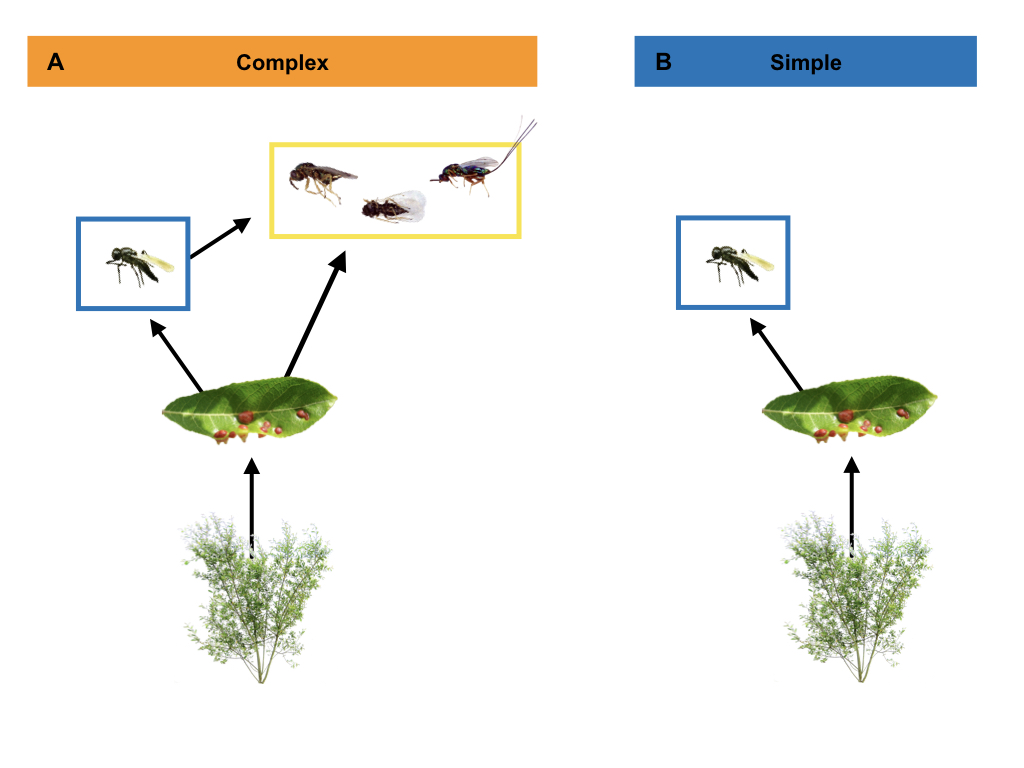
\includegraphics[scale=0.5]{complex_simple_foodwebs.jpeg}
\caption{Illustrations of complex (A) and simple (B) food webs associated with the insect herbivore, \emph{Iteomyia salicisverruca}. Black arrows denote the flow of energy in this network of trophic interactions.}
\label{Fig:Concept}
\end{figure}

\begin{figure}[h!]
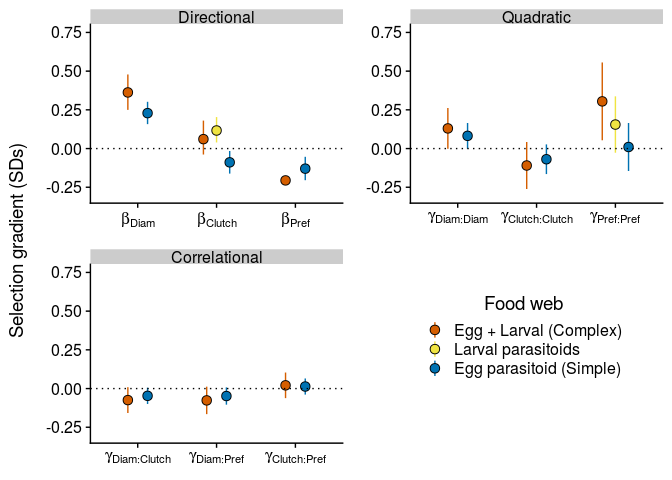
\includegraphics{reproduce_analyses_files/figure-html/Selection-Gradients-1.png}
\caption{Selection gradients acting on \textit{Iteomyia} phenotypes. Points and lines correspond to estimated means and 95\% confidence intervals, respectively. Orange and blue colors correspond to estimated gradients in complex and simple food webs, respectively. Yellow colors correspond to selection gradients imposed by larval parasitoids. Note that we only plot selection gradients for larval parasitoids when they differed from egg parasitoids (simple food web).}
\label{Fig:Gradients}
\end{figure}

\begin{figure}[h!]
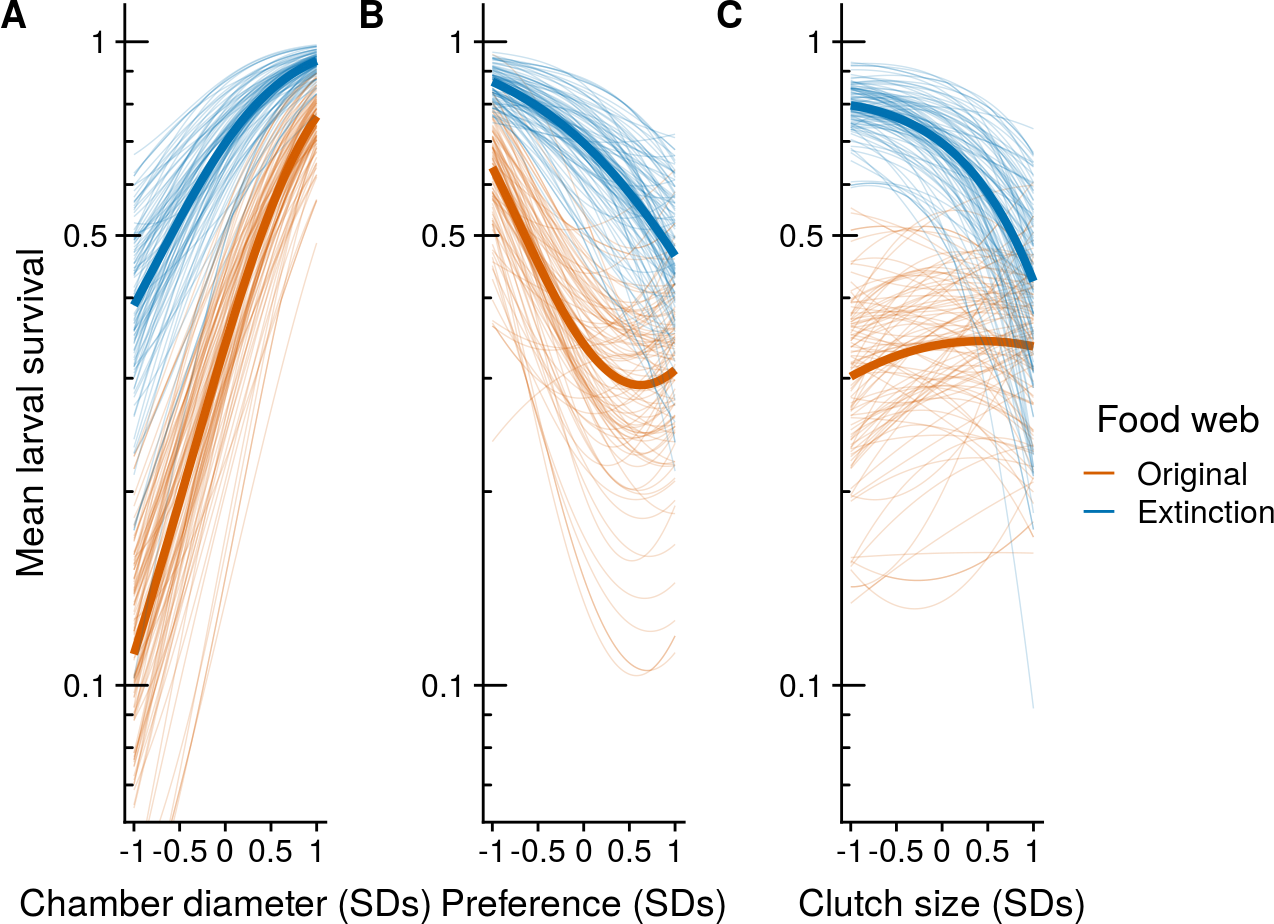
\includegraphics{reproduce_analyses_files/figure-html/Univariate-Fitness-Landscapes-1.png}
\caption{Adaptive landscape of \textit{Iteomyia} phenotypes in complex vs. simple food webs. Each panel corresponds to a different phenotypic trait: chamber diameter (A); clutch size (B); and female preference (C). Solid lines represent the estimated gradients in complex (orange) and simple (blue) food webs. Transparent lines represent bootstrapped replicates to show the uncertainty in estimated gradients. For clarity, we only display 100 bootstraps even though inferences are based on 1,000 bootstrapped samples. Note the mean larva survival is plotted on a natural log scale to accurately reflect the shape of the adaptive landscape.}
\label{Fig:FL_1D}
\end{figure}

\begin{figure}[h!]
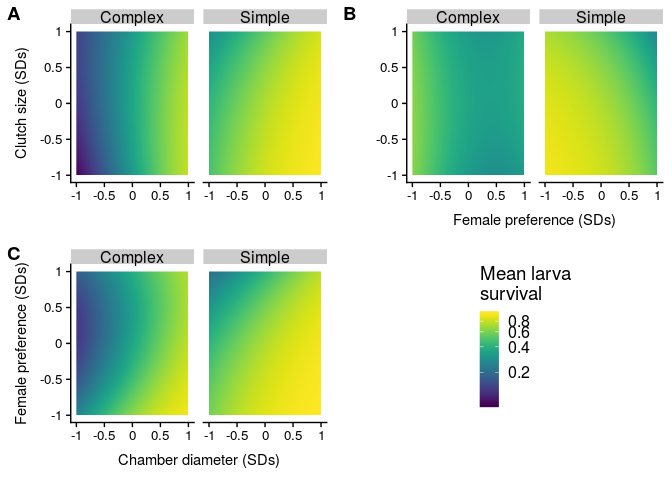
\includegraphics{reproduce_analyses_files/figure-html/Multivariate-Fitness-Landscapes-1.png}
\caption{Two dimensional view of adaptive landscapes in complex vs. simple food webs. Each panel corresponds to a different combination of traits: clutch size and chamber diameter (A); clutch size and female preference (B); female preference and chamber diameter (C). Note the mean larva survival is plotted on a natural log scale to accurately reflect the shape of the adaptive landscape.}
\label{Fig:FL_2D}
\end{figure}


%\subsection*{Online figure legends}

%\renewcommand{\thefigure}{A\arabic{figure}}
%\setcounter{figure}{0}

%\begin{figure}[h!]
%\includegraphics{jumps20m}
%\caption{\textit{A}, the quick red fox proceeding to jump 20~m straight into the air over not one, but several lazy dogs. \textit{B}, the quick red fox landing gracefully despite the skepticism of naysayers.}
%\label{Fig:Jumps}
%\end{figure}

%\begin{figure}[h!]
%\includegraphics{jumps20m}
%\caption{The quicker the red fox jumps, the likelier it is to land near an okapi. For further details, see \citet{LemKapEx07}.}
%\label{Fig:JumpsOk}
%\end{figure}

%\renewcommand{\thefigure}{B\arabic{figure}}
%\setcounter{figure}{0}

\end{document}
